% Chapter 1

\chapter{Introducción} % Main chapter title

\label{hola} % For referencing the chapter elsewhere, use \ref{Chapter1} 

\lhead{\til}
\rhead{\fu}
\lfoot{Chapter 1. \emph{Introducción}} % This is for the header on each page - perhaps a shortened title

%----------------------------------------------------------------------------------------

\section{Introducción}
Históricamente, se ha visto un aumento en la sofisticación, velocidad, impacto y 
cantidad de los ataques informáticos. Se ha vuelto necesario que las estrategias 
de defensa se adapten a los nuevos actores y ataques. Para responder a esto, las 
organizaciones han tenido que recurrir al intercambio de información referente a 
las amenazas con el fin de tener una visión más amplia de las actividades de los 
adversarios y así ayudar a administrar sus recursos de forma de obtener el mejor 
resultado posible de sus defensas. Hoy en día el compartir información es realizado 
de forma manual lo cual es una tarea que consume una cantidad de tiempo 
considerable o por medio de procesos automatizados con grandes limitaciones los 
cuales se realizan dentro de comunidades especificas. La capacidad de compartir 
información completa de forma automática con un gran número de comunidades no 
existe en la actualidad. Hay múltiples métodos para el intercambio de 
información y estos juegan un rol significante en los tipos, volúmenes y 
naturaleza de la información compartida con la comunidad. Algunos de estos 
medios de intercambio limitan el tipo de contenido que es compartido de forma 
sencilla mientras que otros promueven ciertos tipos de intercambio. De todas 
formas, la mayoría de estos métodos no permiten el consumo de información de 
amenazas de forma automática, esto hace que rutinariamente las 
organizaciones deban tomar dicha información y sintetizarla en sus bases de 
datos locales. Si bien los métodos utilizados en la actualidad han ayudado a 
mejorar las capacidades defensivas de numerosas organizaciones, estas no han 
logrado explotar su máximo potencial. Por ello es que actualmente existen varios 
esfuerzos para generar arquitecturas abiertas, estándar basadas en indicadores e 
información de incidentes. La realidad es que ninguno de estos ha podido 
convertirse en un estándar para el intercambio entre comunidades.
Las aproximaciones tradicionales de seguridad se focalizan en entender y 
registrar vulnerabilidades, debilidades y configuraciones necesarias pero 
insuficientes. Para defenderse las organizaciones tienen estrategias de defensa 
que buscan predominantemente bloquear los ataques y arreglar 
las vulnerabilidades, esta estrategia se basa en alertas. Si bien puede ser 
efectiva contra algunas amenazas no logra detener ataques avanzados o proveer 
información sobre las actividades de un atacante luego de que la red fue 
penetrada. Una estrategia mas adecuada es basarse en \emph{cyber kill-chain}, en 
esta estrategia se busca descomponer las fases de un ataque con la finalidad de 
obtener una mejor comprensión del ataque y el atacante así como mejorar las 
posibilidades de defensa.

\begin{figure}[ht!]
  \centering
    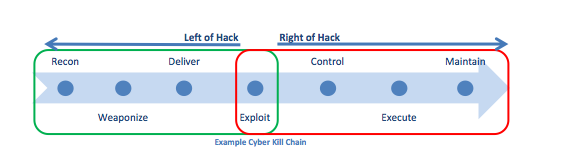
\includegraphics[width=150mm]{./Figures/killChain.png}
\end{figure}

Los primeros pasos de esta estrategia representan una 
oportunidad para detectar y mitigar las amenazas de forma proactiva antes de que 
el adversario realice un acceso no autorizado en los sistemas de la 
organización. En los pasos posteriores es donde se realiza la detección, 
respuesta y aseguramiento de los activos más importantes. Al entender al 
adversario los defensores tienen una mejor oportunidad para descubrir y 
responder al ataque. Un entendimiento de la amenaza permite la realización de 
decisiones mas efectivas, priorizando los recursos para así lograr tener una 
ventaja ante el adversario. El efecto de las defensas en base a inteligencia es 
una mejor postura respecto a las respuestas dado que los atacantes 
ajustan sus operaciones basandose en el éxito o falla de sus intentos. En un 
modelo como el presentado los intentos que realiza un adversario pueden ser 
reconocidos, logrando que los defensores tengan la posibilidad de ajustar sus 
tácticas para una mejor respuesta que genere que el adversario le sea mas 
difícil alcanzar sus objetivos. Compartir información sobre amenazas con socios 
y comunidades de confianza le permite a las organizaciones tener un conjunto de 
información relevante para tener una identificación precisa de una amenaza.
Por el medio de este intercambio, cada ente puede alcanzar un nivel mas alto de 
entendimiento del panorama de las amenazas, no solamente de forma abstracta sino 
que también de evidencias especificas que indiquen la presencia del atacante.
Actualmente se busca que las defensas anticipen y mitiguen 
las amenazas antes de que sean más difíciles de encontrar y erradicar utilizando 
los métodos tradicionales de detección y respuesta. Para poder realizar esto es 
necesario que se realice una actividad de cyber inteligencia recolectando 
información referente a ataques. Con esta información los analistas pueden 
agrupar patrones de actividades similares, atribuir actividades a ciertos 
actores, identificar e implementar estrategias de mitigación de forma rápida y 
anticiparse al lanzamiento de ataques similares en el futuro. Para aprovechar de 
forma más adecuada los beneficios de la cyber inteligencia, las organizaciones 
deben compartir la información recolectada (incluyendo sus estrategias de defensa) 
con socios de su confianza. De esta forma se obtiene una imagen más completa de 
las actividades del adversario y de las acciones defensivas que se deben 
realizar. Por medio del análisis del comportamiento de los adversarios en 
distintos objetivos y en un periodo de tiempo adecuado, los defensores son 
capaces de identificar un conjunto importante de indicadores, tácticas, técnicas 
y procedimientos (TTPs). De esta forma se obtiene información de los objetivos y 
las estrategias lo cual permite al defensor predecir el comportamiento del 
ataque y generar defensas dinámicas. Dada la forma y complejidad con la que 
evoluciona el panorama de las amenazas, la velocidad con la cual ocurren los 
eventos, y la basta cantidad de datos que se deberian intercambiar, es necesario 
establecer una forma automática para ayudar a los analistas y tomadores de 
decisión a tomar acciones defensivas para que esta aproximación sea efectiva. La 
automatización requiere de información de calidad, dado que las arquitecturas 
son heterogéneas con distintos productos y sistemas, es necesario la 
estandarización con representaciones estructuradas de información y un mejor 
aprovechamiento de la información sin saber de antemano quien va a proveer que 
información. Dicha información debe ser legible por un humano y pareseable por 
una máquina. Estos requerimientos tienen varias justificaciones, primer que 
nada, un analista podría realizar un análisis que es inapropiado para ser 
automatizado o que sea focalizados en tomas de decisiones por parte de personas. 
También podría ser de interés que un analista tenga conocimiento de la situación 
actual. Además podría ser un buen medio para evaluar la fidelidad de las fuentes 
y los métodos utilizados para producir la información. Dados todos los factores 
presentados anteriormente, es necesaria la existencia de representaciones 
estructuradas de la información y que esta sea expresiva, flexible, extensible, 
automatizable y legible. Además se deben contar con medios para permitir el 
intercambio seguro y confiable de información entre distintas organizaciones.



